% Standalone preview wrapper for local compilation.
% When merging into the main report, paste the content beginning at
% "\subsection{Firmware}" and omit this preamble/document wrapper.
\documentclass[conference]{IEEEtran}
\usepackage{graphicx}
\usepackage{tabularx}
\usepackage{xcolor}
\usepackage{hyperref}

\begin{document}

\section{Design Strategy}

\subsection{Firmware}

The vehicle firmware is built around a Raspberry Pi Pico based control layer that bridges high-level autonomy commands to low-level hardware interfaces. Its primary role is to provide deterministic actuation, safety monitoring, and sensor/telemetry exchange while remaining reusable across multiple MRG boards. Rather than treating each embedded target as a separate codebase, the firmware was intentionally structured as a configurable product line so that new boards can inherit common infrastructure while selecting only the interfaces they require.

\subsubsection{Firmware Architecture}

The firmware is organized as a shared embedded framework with board-specific application classes. At compile time, a selected PlatformIO environment instantiates one board class in \texttt{main.cpp}, and that class defines the setup and update flow for the target hardware. This keeps the top-level application logic simple while allowing different hardware variants to reuse the same module library for motor control, emergency stop handling, sensing, indicator outputs, and communications.

The design separates responsibilities into reusable modules. Safety interfaces are encapsulated in the E-stop and leak-sensing components, actuation is grouped in the motor and dropper control modules, sensor drivers are isolated from the application flow, and transport logic for telemetry and command exchange is handled through dedicated Protocol Buffers sender and receiver classes. This structure reduces duplication and makes it practical to reuse code between the AUV motor interface board, sensing board, and firmware test targets without rewriting the full application stack for each revision.

\subsubsection{Configurable Multi-Board Support}

One of the main firmware design goals was to support multiple hardware variants from a single repository. This is implemented through PlatformIO build environments and board-specific compile flags. Each environment enables only the features needed for a given target, such as motors, sensor buses, LED outputs, dropper control, or protocol messaging. The result is a single codebase that can be compiled into several board personalities without maintaining separate branches for each board.

\begin{table}[htbp]
\caption{Representative firmware targets supported by the shared codebase.}
\label{tab:firmware_targets}
\begin{center}
\begin{tabularx}{\columnwidth}{|p{0.23\columnwidth}|p{0.24\columnwidth}|X|}
\hline
\textbf{Build Target} & \textbf{Primary Role} & \textbf{Key Enabled Capabilities} \\
\hline
\texttt{board\_alpha} / Presto demo & Generic motor interface validation & Motor outputs, LED mux, indicator outputs, emergency stop logic \\
\hline
\texttt{board\_beta} / Sensor demo & Sensor-side proof of concept & I2C sensing, status indication, emergency stop logic \\
\hline
\texttt{boat\_presto\_jr} / \texttt{board\_delta} & Proto communication board & Protocol transport, E-stop state exchange, board-level command handling \\
\hline
\texttt{sub\_presto} / \texttt{board\_epsilon} & RoboSub motor interface board & Eight-thruster command output, dropper actuation, LED mux, autonomy switch, protocol messaging, emergency stop logic \\
\hline
\texttt{sensor\_demo\_zeta} and RTOS variant & Sensor framework validation & Inheritance-based sensor interface, protocol telemetry, optional RTOS-oriented template \\
\hline
\end{tabularx}
\end{center}
\end{table}

This configurable approach is especially valuable for a student team supporting several concurrent embedded efforts. Common software infrastructure can mature in one project and then be carried into another with much lower integration cost. It also simplifies debugging because the team can bench-test a reduced feature set on dedicated demo targets before deploying the same interfaces on the full vehicle board.

\subsubsection{Real-Time I/O and Actuation}

The firmware makes deliberate use of the RP2040's Programmable I/O (PIO) peripheral to offload timing-sensitive or repetitive digital behavior from the CPU. Within the current implementation, PIO is used to demonstrate LED timing and multiplexed output patterns, serving both as a practical subsystem and as a proof of concept for more advanced offloaded interfaces. This matters because the embedded controller must eventually service command handling, actuation updates, safety state changes, and telemetry simultaneously. Offloading repetitive signaling to dedicated PIO state machines preserves CPU time for control-critical logic.

Motor and actuator outputs are handled separately from the PIO demonstration features. Early servo control approaches consumed scarce PIO state machine resources, which limited scalability. The firmware was therefore migrated to a hardware PWM based servo library for sustained actuator control. This change freed PIO resources for future communications and timing applications while also enabling the addition of more outputs, including the dropper actuator required for RoboSub task execution. In practice, this means the shared motor interface board can command the vehicle thrusters while also supporting extra payload actuators without exhausting low-level peripheral resources.

\subsubsection{Safety and Fault Response}

Safety behavior is treated as a first-class firmware concern rather than an afterthought layered on top of command logic. The firmware includes emergency stop interfaces that can immediately inhibit actuation in response to kill-switch or fault conditions, and the board-level application classes are written so that safety status remains globally visible. This is important for a competition vehicle because autonomy, operator commands, and safety interlocks all contend for authority over the same outputs. The firmware therefore centralizes the decision of whether actuators are allowed to run while still keeping individual modules self-contained.

The same structure is extensible to additional safety triggers such as leak detection and watchdog-based fault handling. Even where those interfaces are still evolving, the architecture already reflects the intended behavior: safety signals should be simple to read, easy to propagate through the application, and able to override normal actuation logic with minimal latency.

\subsubsection{Sensor Interfaces and Data Abstraction}

The sensing side of the firmware demonstrates the transition from one-off drivers to a more reusable abstraction model. Current implementations include I2C-connected environmental and inertial sensors, specifically a temperature/humidity sensor and a 9-DOF IMU class used as a stand-in for more complete sensing-board functionality. These devices share common setup and readback patterns, and newer demo targets wrap them behind a common \texttt{Sensor} parent interface. That interface defines standard behavior for initialization, emergency stop handling, and data acquisition, which gives downstream code a more predictable way to consume measurements.

This abstraction is useful beyond code cleanliness. By forcing different sensors to present a common interface, the firmware can support templated board implementations, standardized telemetry packaging, and future substitution of real mission sensors without rewriting the application structure. It also provides a cleaner path toward RTOS-based task separation because each sensor can evolve into an independent periodic task while preserving the same external API.

\subsubsection{ROS and Protocol Buffers Integration}

A major firmware milestone was the development of a lightweight transport bridge between the Pico and the vehicle's ROS 2 software stack. The repository includes a Protocol Buffers schema, generated nanopb message wrappers, and dedicated sender and receiver classes that serialize commands and telemetry over a framed serial transport. On the host side, matching Python tools are provided for dry testing and debugging, allowing developers to inject motor or actuator commands and inspect firmware responses without requiring the full vehicle software stack.

For RoboSub specifically, this communication layer allows high-level autonomy and controls software running on the Jetson to command the motor interface board using structured messages rather than ad hoc byte streams. The firmware receiver decodes incoming messages into motor commands, dropper commands, manual-mode state, and other control fields, while the sender supports status and telemetry messages in the opposite direction. This creates a cleaner contract between embedded and high-level software, reduces parsing ambiguity, and makes it easier to grow the command vocabulary as the vehicle gains more subsystems.

\subsubsection{Development Workflow and Verification}

The firmware project was also designed to be practical for student development, not only for deployment. Build-time scripts automatically generate PIO wrapper headers and Protocol Buffers support files, reducing the chance of hand-maintained interface drift. The repository includes multiple demo environments for feature validation, Python-based serial test tools for dry testing, and Pico Probe compatible debug targets for cases where standard USB serial output is already occupied by the protocol bridge. Together, these tools support a workflow in which new hardware features can be bench-tested in isolation before being integrated into the full vehicle.

The strongest example of this dry-test philosophy is the terminal-based validation tool built with the Blessed Python library. That interface turns the firmware link into an interactive bench-testing console rather than a passive serial monitor. It automatically discovers the Pico over USB, maintains a framed Protocol Buffers session, and displays command and telemetry state in real time. Because the interface is visual, low-latency, and easy to operate during hardware bring-up, it significantly lowers the barrier to testing firmware changes on a desk before attempting full system integration.

\begin{figure*}[htbp]
\centering
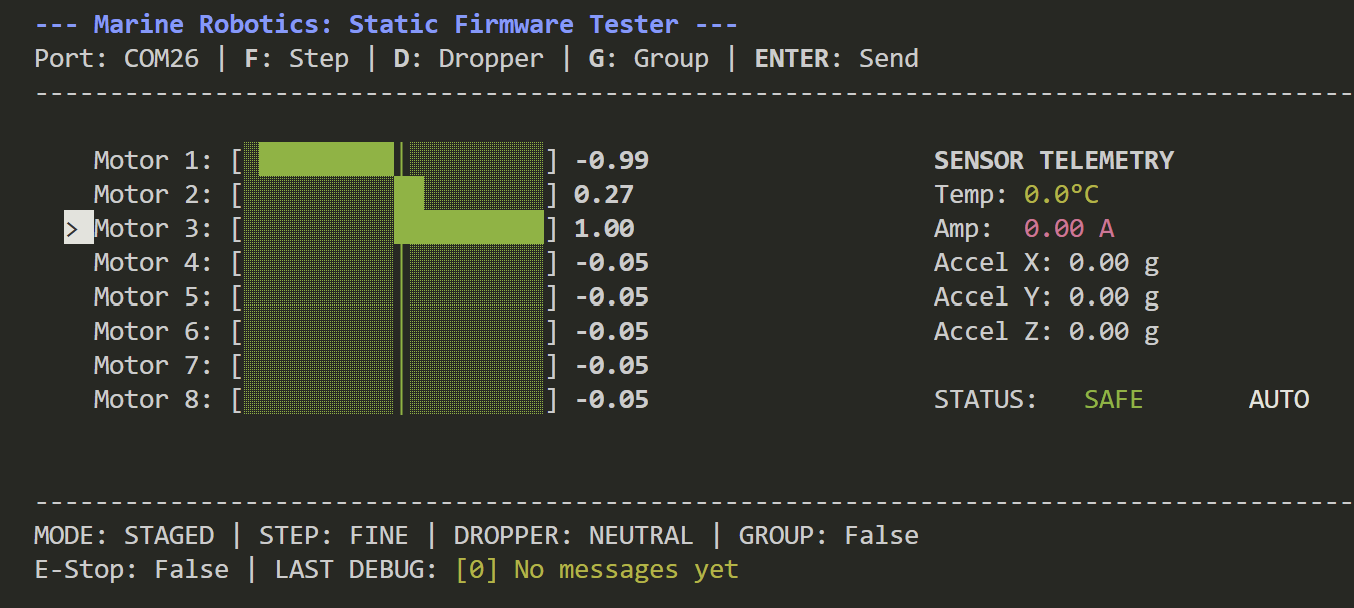
\includegraphics[width=0.92\textwidth]{pictures/testbench.png}
\caption{Blessed-based static firmware tester used for dry validation of command transport, motor and dropper actuation, telemetry parsing, and returned firmware status. The interface presents live actuator commands, sensor telemetry, system mode, and the most recent debug message in a single operator-facing view.}
\label{fig:firmware_testbench}
\end{figure*}

\begin{table}[htbp]
\caption{Capabilities exercised by the Blessed-based firmware tester.}
\label{tab:blessed_tester}
\begin{center}
\begin{tabularx}{\columnwidth}{|p{0.24\columnwidth}|X|}
\hline
\textbf{Tested Feature} & \textbf{Why It Matters} \\
\hline
Automatic serial discovery & Reduces setup error during bench testing and makes it easier for new team members to connect to the correct Pico without manual port hunting. \\
\hline
Heartbeat-based motor command streaming & Verifies that the firmware continues to receive fresh commands at a fixed cadence, which is critical for confirming that actuators fail predictably if communications stall. \\
\hline
Independent eight-motor control & Confirms correct motor-channel mapping, command scaling, sign convention, and per-thruster response before the full vehicle is placed in the water. \\
\hline
Grouped motor control & Allows all motors to be stepped together, which is useful for validating symmetric drive behavior and quickly checking whether the board responds consistently under common commands. \\
\hline
Fine and coarse command stepping & Supports both detailed tuning and rapid sweeps, making it possible to observe deadband, saturation, and response smoothness without modifying firmware between tests. \\
\hline
Live mode and staged mode & Distinguishes between editing commands locally and transmitting them immediately, which helps prevent accidental actuation while still enabling rapid closed-loop bench validation. \\
\hline
Sine-wave command mode & Exercises continuously varying outputs and is useful for exposing timing glitches, jitter, or unstable command handling that may not appear during static tests. \\
\hline
Zeroing and neutral command reset & Provides a quick way to return all outputs to a safe known state, which is important whenever actuators are being tested on the bench. \\
\hline
Dropper command cycling & Verifies payload actuation states and confirms that auxiliary outputs beyond the main thruster set are correctly serialized, transmitted, and executed. \\
\hline
E-stop and manual/auto status display & Confirms that critical system state is making the return trip from firmware to host, allowing operators to verify that safety and mode logic are behaving as intended. \\
\hline
Debug message display with identifiers & Makes embedded execution more observable even when standard serial printing is limited, which speeds debugging of protocol handling and board logic. In the current implementation these identifiers act as message tags for distinguishing firmware outputs; they align naturally with future query-oriented workflows, but they are not yet used by the present tester as incoming query selectors. \\
\hline
Telemetry display for temperature, current, and acceleration & Demonstrates that sensor packets are encoded, transmitted, decoded, and rendered correctly, which is a necessary precursor to trustworthy health monitoring and downstream autonomy use. \\
\hline
\end{tabularx}
\end{center}
\end{table}

This tester is valuable not only because it checks many interfaces at once, but because it checks the exact interfaces that most often fail during embedded integration: command formatting, packet framing, actuator mapping, telemetry interpretation, and operator visibility into system state. The debug identifiers are part of that observability strategy. In the current code they are attached to outgoing debug messages, and similar identifier fields are also used on sensor telemetry packets to distinguish reported data types. That means the present implementation already supports structured classification of returned information, even though it does not yet implement a host-side mechanism that queries subsystems by debug identifier alone. In other words, it validates the complete chain from host-side message generation to firmware-side execution and back to host-side feedback. For a robotics team with limited water-test opportunities, that kind of end-to-end bench validation is especially important because it moves many failures out of the pool and onto the workbench, where they are faster, safer, and cheaper to diagnose.

This workflow directly supports the team's broader competition strategy. Pool time is limited and expensive, so firmware failures must be detected as early as possible on the bench. By validating command transport, safety behavior, actuator outputs, and sensor formatting in dry tests, the team reduces the number of integration issues that appear only once the vehicle is in the water.

\subsubsection{Current Maturity and Contribution to the Vehicle}

At its current level of maturity, the firmware foundation is more than a basic proof of concept but intentionally less than a finished embedded product line. The essential pieces needed for RoboSub integration are already present: multi-board configuration, structured host communication, motor and dropper actuation, emergency stop handling, representative sensing interfaces, and a repeatable testing workflow. Just as importantly, the framework leaves room for future expansion into DMA-assisted transport, more advanced PIO communication engines, broader sensing-board support, and RTOS-based scheduling without forcing a redesign of the entire codebase.

Within the overall AUV system, the firmware therefore serves two purposes. First, it is the immediate embedded control layer that makes the current motor interface and sensing hardware usable by the vehicle. Second, it is a reusable foundation for future MRG projects that need safe, modular, and ROS-compatible embedded control on Raspberry Pi Pico class hardware.

\end{document}
